% Gini coefficient of one gene across cell types, vignette 03-1,
% #fig-gini-derivation (#sec-gini-entropy, eq-gini).
% Panels: scripts/figures/fig_03_1_gini.R (ggplot2; identities checked there).
% Build: latexmk -lualatex gini.tex; pdftocairo -svg gini.pdf ../../fig_03_1_gini.svg
%        pdftocairo -png -r 200 -singlefile gini.pdf ../../fig_03_1_gini
\documentclass[tikz,border=4pt]{standalone}
\usepackage{iftex}
\ifPDFTeX
  \PackageError{gini}{Use LuaLaTeX or XeLaTeX}{}
\fi
\usepackage{fontspec}
\usepackage{amsmath,amssymb,amsfonts,bm}
\usepackage{graphicx}
\usepackage{awesomebox} % loads fontawesome5
\usetikzlibrary{arrows.meta,positioning,fit,backgrounds,calc,shapes.geometric}
% palette and flowchart styles of vignettes/_quarto.yml
\definecolor{ink}{HTML}{1F2937}
\definecolor{latfill}{HTML}{DAE9FB}
\definecolor{latdraw}{HTML}{4477B5}
\definecolor{obsfill}{HTML}{C9CDD3}
\definecolor{obsdraw}{HTML}{747B86}
% the two example genes (series colours of the R panels)
\definecolor{lowgene}{HTML}{1D4E89}
\definecolor{highgene}{HTML}{C45C26}
\tikzset{
  every node/.style={text=ink},
  edge/.style={-{Stealth[length=2.6mm]}, line width=0.8pt, draw=ink},
  box/.style={rectangle, rounded corners=3pt, draw=ink, fill=white, line width=0.8pt,
    align=flush left, inner sep=1.6mm, font=\small},
  keybox/.style={box, draw=latdraw, fill=latfill},
  stepnode/.style={box, draw=latdraw, fill=latfill!35, inner sep=1.8mm,
    text width=\stepw, minimum height=\rowh},
  panel/.style={inner sep=0pt, anchor=west},
  tag/.style={font=\bfseries\small, anchor=north west, inner sep=1pt}
}
% geometry: rows of the height of one R panel (3.4 x 1.4 in; row E 3.4 x 1.6 in)
\newlength{\stepw}\setlength{\stepw}{8.3cm}
\newlength{\rowh}\setlength{\rowh}{1.4in}
\newlength{\rowhE}\setlength{\rowhE}{1.6in}
\newlength{\iconw}\setlength{\iconw}{1.15cm}
\newlength{\rulew}\setlength{\rulew}{1.2pt}
\newsavebox{\stepcontent}
\newsavebox{\stepicon}
% \stepbox{letter}{icon}{title}{formula (display maths)}{explanation}
% awesomebox: icon column of width \iconw, vertical rule, content column;
% the icon is lowered so that its centre sits at the centre of the content.
\newcommand{\stepbody}[4]{%
  \begingroup\raggedright % grouped: \raggedright redefines the row end \\
  \textbf{#1\enspace #2}\par
  \setlength{\abovedisplayskip}{2pt}\setlength{\belowdisplayskip}{2pt}%
  \setlength{\abovedisplayshortskip}{2pt}\setlength{\belowdisplayshortskip}{2pt}%
  #3\par
  {\footnotesize #4\par}\endgroup}
\newcommand{\stepbox}[5]{%
  \begin{minipage}{\stepw}\small
    \setlength{\aweboxvskip}{0pt}%
    \setlength{\aweboxleftmargin}{\iconw}%
    \setlength{\aweboxlinewidthref}{\linewidth}%
    \setlength{\aweboxcontentwidth}{\dimexpr\linewidth-\iconw\relax}%
    \sbox{\stepcontent}{\parbox[t]{\dimexpr\aweboxcontentwidth-\rulew-\tabcolsep\relax}%
      {\stepbody{#1}{#3}{#4}{#5}}}%
    \sbox{\stepicon}{\Huge #2}%
    \setlength{\aweboxsignraise}{%
      \dimexpr-0.5\ht\stepicon+0.5\ht\stepcontent-0.5\dp\stepcontent\relax}%
    \awesomebox[latdraw]{\rulew}{#2}{latdraw}{\stepbody{#1}{#3}{#4}{#5}}%
  \end{minipage}}
\begin{document}
\begin{tikzpicture}
  \def\pitch{4.25} % row height (3.56 cm) plus the gap for the arrows, in cm
  \def\xpanel{9.25}
  \def\yE{-4*\pitch-0.254} % row E is 0.2 in taller: centre lowered by 0.1 in
  % ---- step boxes --------------------------------------------------------
  \node[stepnode, anchor=west] (bA) at (0,0) {\stepbox{A}{\faArrowsAltH}%
    {Pairwise inequality}%
    {\[\Delta_g=\frac{1}{J^{2}}\sum_{j=1}^{J}\sum_{\ell=1}^{J}
      \lvert\mu_{gj}-\mu_{g\ell}\rvert\]}%
    {Mean absolute difference of the type means $\mu_{gj}$; in counts,
    so it doubles when every $\mu_{gj}$ doubles.}};
  \node[stepnode, anchor=west] (bB) at (0,-\pitch) {\stepbox{B}{\faBalanceScale}%
    {Scale-free}%
    {\[\mathrm{Gini}_g=\frac{\Delta_g}{2\bar\mu_g},\qquad
      \bar\mu_g=\frac{1}{J}\sum_{j=1}^{J}\mu_{gj}\]}%
    {Dividing by twice the mean leaves $\mathrm{Gini}_g$ unchanged when all
    means are multiplied by a constant $c>0$.}};
  \node[stepnode, anchor=west] (bC) at (0,-2*\pitch) {\stepbox{C}{\faSortAmountUp}%
    {Ordering}%
    {\[\mathrm{Gini}_g=\frac{1}{J^{2}\bar\mu_g}\sum_{j=1}^{J}(2R_{gj}-J-1)\,\mu_{gj}\]}%
    {$R_{gj}$: rank of $\mu_{gj}$; order statistics $\mu_{g(1)}\le\cdots\le\mu_{g(J)}$. One weighted sum
    over $J$ sorted means replaces the $J^{2}$ pairs. Panel: the sum over
    $J^{2}\bar\mu_g=800$.}};
  \node[stepnode, anchor=west] (bD) at (0,-3*\pitch) {\stepbox{D}{\faRulerHorizontal}%
    {Finite-$J$ correction}%
    {\[\max\mathrm{Gini}_g=\frac{J-1}{J},\qquad
      \frac{J}{J-1}\,\mathrm{Gini}_g\in[0,1]\]}%
    {Reached when one type carries all the mass (grey row);
    the rescaled score of that gene is 1.}};
  \node[stepnode, anchor=west, minimum height=\rowhE] (bE) at (0,\yE) {\stepbox{E}{\faChartPie}%
    {Shares $u_{gj}=\mu_{gj}\big/\sum_{\ell}\mu_{g\ell}$}%
    {\[\begin{aligned}
      \mathrm{Gini}_g
      &=\frac{1}{2J}\sum_{j=1}^{J}\sum_{\ell=1}^{J}\lvert u_{gj}-u_{g\ell}\rvert\\
      &=\frac{1}{J}\sum_{j=1}^{J}(2R_{gj}-J-1)\,u_{gj}
    \end{aligned}\]}%
    {Since $u_{gj}=\mu_{gj}/(J\bar\mu_g)$, B and C give this value.}};
  \foreach \a/\b in {bA/bB,bB/bC,bC/bD,bD/bE}
    \draw[edge] (\a.south) -- (\b.north);
  % ---- panels, one per step, on the same row --------------------------------
  \node[panel] (pA) at (\xpanel,0) {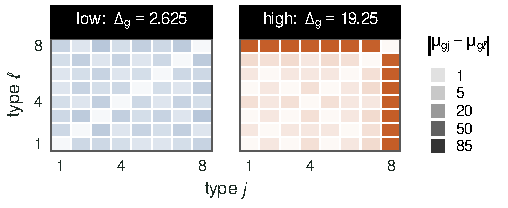
\includegraphics[width=3.4in]{panel_a_pairwise.pdf}};
  \node[panel] (pB) at (\xpanel,-\pitch) {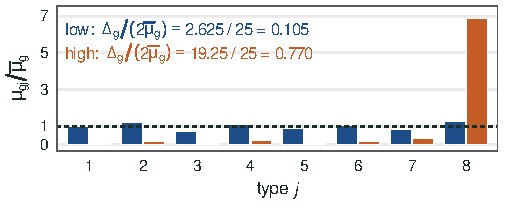
\includegraphics[width=3.4in]{panel_b_scale_free.pdf}};
  \node[panel] (pC) at (\xpanel,-2*\pitch) {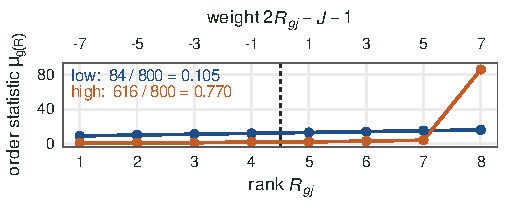
\includegraphics[width=3.4in]{panel_c_ordering.pdf}};
  \node[panel] (pD) at (\xpanel,-3*\pitch) {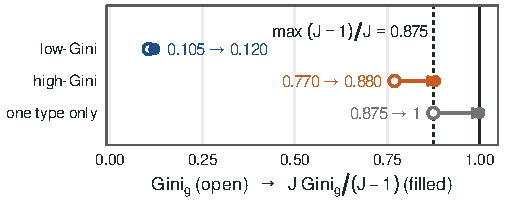
\includegraphics[width=3.4in]{panel_d_correction.pdf}};
  \node[panel] (pE) at (\xpanel,\yE) {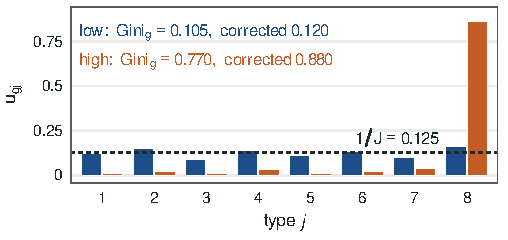
\includegraphics[width=3.4in]{panel_e_shares.pdf}};
  \foreach \p/\t in {pA/A,pB/B,pC/C,pD/D,pE/E}
    \node[tag] at ($(\p.north west)+(-0.38,0)$) {\t};
  % ---- data key --------------------------------------------------------------
  \path (bA.west |- bA.north) ++(0,0.35) coordinate (keySW);
  \node[keybox, anchor=south west, text width=17.45cm] (key) at (keySW)
    {Gene $g$ fixed, $J=8$ cell types $j,\ell$, type means (counts) $\mu_{gj}$;
    both genes have $\bar\mu_g=12.5$ and every $\mu_{gj}\ge1$.\\[1pt]
    \textcolor{lowgene}{\rule{2.4mm}{2.4mm}}\ low-Gini gene
    $\mu_{g\cdot}=(12,15,9,14,11,13,10,16)$\qquad
    \textcolor{highgene}{\rule{2.4mm}{2.4mm}}\ high-Gini gene
    $\mu_{g\cdot}=(1,2,1,3,1,2,4,86)$};
\end{tikzpicture}
\end{document}
